\dr{
About the corpus origins, aims, format.
}

\begin{itemize}
    \item Size
        \begin{itemize}
            \item 7545103 XML files in 48,482 directories comprising 2,271,985,142 words and 32.7952GiB of data [inc markup].
            \item Word sizes: 40, 83, 147, 308, 1400 at 5\%, 25\%, 50\%, 75\% and 95\%.
            % > quantile(words$words, c(.05, .25, .50, .75, .95))
            %   5%  25%  50%  75%  95% 
            %   40   83  147  308 1400
            \item Average filesize is 2.4KB
            \item Totals and breakdowns
        \end{itemize}
    \item Format
        \begin{itemize}
            \item Individual files
            \item folder structure and organisation (pertinent to later organisation/batching)
        \end{itemize}
\end{itemize}

\subsection{Format}
The corpus is split into 7,545,103 XML files, each representing a speech made in either house of the UK Parliament.  These files are organised into a hierarchical directory structure by house and date.  A sample of this structure is shown in Figure~\ref{fig:structure}.

\begin{figure}[h]
    \centering
    {
        \small
        \begin{Verbatim}[frame=single]
            Hansard
            +-- Commons
            |   +-- commons 1803-1820
            |   |   \-- commons
            |   |       +-- 1803
            |   |       |   +-- dec
            |   |       |   |   +-- 01
            |   |       |   |   +-- 02
            |   |       |   |   +-- 03
            |   |       |   |   +-- 05
            |   |       |   |   +-- ...
        \end{Verbatim} 
    }
    \caption{Sample directory layout}
    \label{fig:structure}
\end{figure}


\begin{figure}[h]
    \centering
    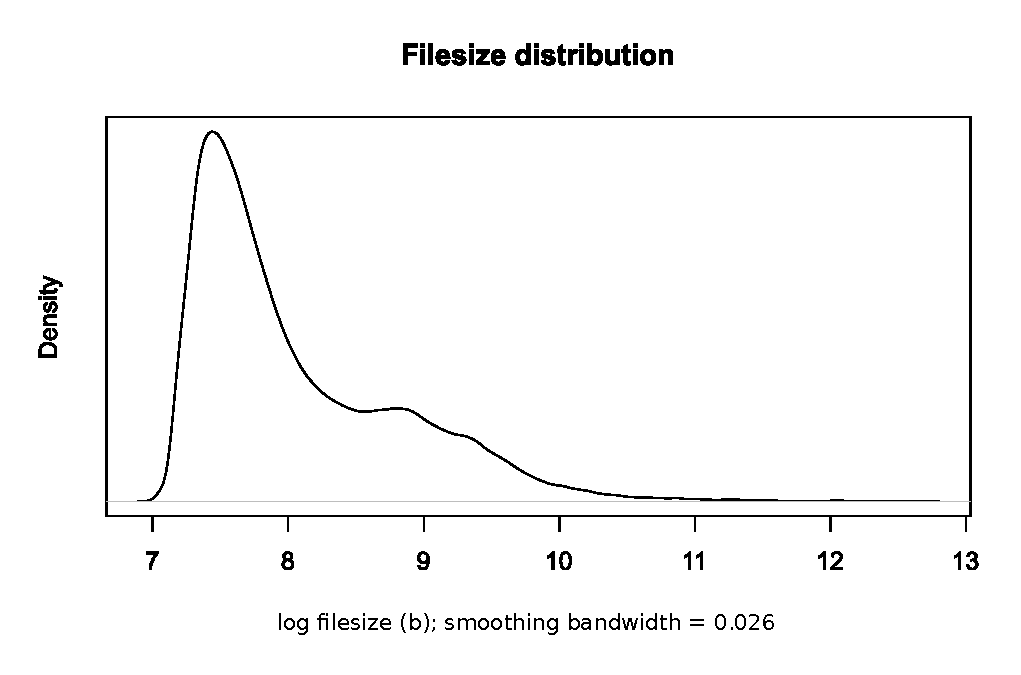
\includegraphics[width=0.5\textwidth]{filesize.eps}


    \begin{tabular}{ | r | c | c | c | c | c | }
        \hline
        Percentile & 5 & 25 & 50 & 75 & 95 \\ \hline
        Words & 40 & 83 & 147 & 308 & 1400 \\ \hline
    \end{tabular}

    \caption{Distribution of log filesizes for all corpus data, and word counts (without markup) for each file.}
    \label{fig:filesizes}
\end{figure}


\dr{The XML format used contains annotations for X, Y and Z, and follows various conventions...  }

The XML files themselves follow x format\todo{unsure of this, SW}. File sizes are distributed in a Zipfian manner, as shown in Figure~\ref{fig:filesizes}. The median size is just 2.4KB, and the 95th percentile is 1.4MB.


% \begin{verbatim}
% > quantile(sizes$filesize, c(.05, .25, .50, .75, .95))
%    5%   25%   50%   75%   95% 
%  1411  1781  2443  5031 14013
% \end{verbatim}


\subsection{Tagging}
\begin{itemize}
    \item What needed tagging
    \item Which frequencies had to be built (per file/day/totals)
    \item What work this contributed to
\end{itemize}
